% DOC SETTINGS ===================================
\documentclass{article}
\usepackage[utf8]{inputenc}
\usepackage{steinmetz}
\usepackage{mathtools}  
\usepackage{multicol}
\usepackage{circuitikz}
\usepackage{listings}
\usepackage{geometry}
\usepackage{fancyhdr}
\pagestyle{fancy}
\lhead{ECE2214 Homework 2}
\rhead{Kavin Thirukonda 2021}
\fancyheadoffset{0mm}
\geometry{
 a4paper,
 total={170mm,257mm},
 left=20mm,
 top=25mm,
 }
\mathtoolsset{showonlyrefs} 
\cfoot{}
% DOC SETTINGS ===================================
\begin{document}
\begin{enumerate}
    \item A NMOS transistor with $V_{TN} = 1V$ has a drain current $i_D = 0.8mA$ when $v_{GS} = 3V$ and $v_{DS} = 4.5V$. Calculate the drain current when:
    \begin{center}
        Since $v_{DS} = 4.5V$, $v_{DS}(sat) = 2V$, and $v_{DS} > v_{DS}(sat)$ the transistor is in saturation for the initial conditions, therefore we can use the saturation formula and the given values to solve for unknowns:
    \end{center}
    \begin{align}
        i_D &= K_n(v_{GS} - V_{TN})^2\\
        \Rightarrow 0.8mA &= K_n(3V - 1V)^2\\
        \Rightarrow K_n &= \frac{0.8mA}{(2V)^2}\\
        \Rightarrow K_n &= 0.2\frac{mA}{V^2}\\
    \end{align}
    \begin{enumerate}
        \item $v_{GS} = 2V$, $v_{DS} = 4.5V$
        \begin{center}
            Since $v_{DS} = 4.5V$, $v_{DS}(sat) = 1V$, and $v_{DS} > v_{DS}(sat)$ the transistor is in saturation. Which means we can use the saturation current formula to solve for the current.
        \end{center}
        \begin{align}
            i_D &= K_n(v_{GS} - V_{TN})^2\\
            &= 0.2\frac{mA}{V^2}(2V - 1V)^2\\
            &= 0.2\frac{mA}{V^2}(1V^2)\\
            &= \boxed{0.2mA}
        \end{align}
        \item $v_{GS} = 3V$, $v_{DS} = 1V$
        \begin{center}
            Since $v_{DS} = 1V$, $v_{DS}(sat) = 2V$, and $v_{DS} < v_{DS}(sat)$ the transistor is in non-saturation. Which means we can use the non-saturation current formula to solve for the current.
        \end{center}
         \begin{align}
            i_D &= K_n[2(v_{GS} - V_{TN})v_{DS} - v^2_{DS}]\\
            &= 0.2\frac{mA}{V^2}[2(3V - 1V)1V - (1V^2)]\\
            &= 0.2\frac{mA}{V^2}[4V^2 - 1V^2]\\
            &= \boxed{0.6mA}
        \end{align}
    \end{enumerate}
    \newpage
    \item A PMOS transistor with $V_{TP} = -1.2V$ has a drain current $i_D = 0.5mA$ when $v_{SG} = 3V$ and $v_{SD} = 5V$. Calculate the drain current when:
    \begin{center}
        Since $v_{SD} = 5V$, $v_{SD}(sat) = 1.8V$, and $v_{SD} > v_{SD}(sat)$ the transistor is in saturation for the initial conditions, therefore we can use the saturation formula and the given values to solve for unknowns:
    \end{center}
    \begin{align}
        i_D &= K_p(v_{SG} + V_{TP})^2\\
        \Rightarrow 0.5mA &= K_p(3V-1.2V)^2\\
        \Rightarrow K_p &= \frac{0.5mA}{(1.8V)^2}\\
        \Rightarrow K_p&= 0.1543\frac{mA}{V^2}
    \end{align}
    \begin{enumerate}
        \item $v_{SG} = 2V,v_{SD} = 3V$
        \begin{center}
            Since $v_{SD} = 3V$, $v_{SD}(sat) = 0.8V$, and $v_{SD} > v_{SD}(sat)$ the transistor is in saturation. Which means we can use the saturation current formula to solve for the current.
        \end{center}
        \begin{align}
            i_D &= K_p(v_{SG} + V_{TP})^2\\
            &= 0.1543\frac{mA}{V^2}(2V -1.2V)^2\\
            &= 0.1543\frac{mA}{V^2}(0.8V)^2\\
            &= \boxed{.0987mA}
        \end{align}
        \item $v_{SG} = 5V,v_{SD} = 2V$
        \begin{center}
            Since $v_{SD} = 2V$, $v_{SD}(sat) = 3.8V$, and $v_{SD} < v_{SD}(sat)$ the transistor is in non-saturation. Which means we can use the non-saturation current formula to solve for the current.
        \end{center}
        \begin{align}
            i_D &= K_p[2(v_{SG} + V_{TP})v_{SD} - v^2_{SD}]\\
            &= 0.1543\frac{mA}{V^2}[2(5V - 1.2V)2V - 2V^2]\\
            &=  0.1543\frac{mA}{V^2}[15.2V^2 - 4V^2]\\
            &= \boxed{1.73mA}
        \end{align}
    \end{enumerate}
    \newpage
    \item The transistor below has parameters $ V_{TN} = 0.35V$ and $K_n = 25 \mu A/V^2$. The circuit parameters are $V_{DD} = 2.2V$, $R_1 = 355k\Omega, R_2 = 245k\Omega$, and $R_D = 100k\Omega$. Find $I_D, V_{GS},$ and $V_{DS}$.
    \begin{center}
        \begin{circuitikz}[american voltages]
            \draw (0,0) to [short, i>_=0](2.01,0);
            \ctikzset{tripoles/mos style/arrows}
            \draw (3,0) node[nmos]{};
            \draw (0,0) to [R,l=$R_1$](0,3)
            to [short](3,3)
            to [R, l=$R_D$, i>_=$i_D$](3,.777);
            \draw (0,0) to [R, l=$R_2$](0,-3)
            to [short](3,-3)
            to [short](3,-.777);
            \draw (1.5, 3) to[short, -o,l=$+V_{DD}$](1.5, 3.5);
            \draw (1.5, -3) node[ground]{};
            \draw (3,-1.5) to [open, v=$V_{GS}$](1.5,0);
            \draw (3.25,1.1) to [open, v=$V_{DS}$](3.25,-1.1);
        \end{circuitikz}
    \end{center}
    \begin{equation}
        v_{GS} = 2.2V\frac{245k\Omega}{355k\Omega+245k\Omega} = \boxed{898mV}
    \end{equation}
    \begin{center}
        Since the voltage $v_{GS}$ is greater than the threshold voltage $v_{TN}$ we can see that the device is on.The next step is to assume that the device is in saturation and try to confirm that answer afterwards.
    \end{center}
    \begin{align}
        i_D &= K_n(v_{GS} - V_{TN})^2\\
        &= 25\frac{\mu A}{V^2}(.898V  - 0.35V)^2\\
        &= 25\frac{\mu A}{V^2}(0.3V^2)\\
        &= \boxed{7.517\mu A}
    \end{align}
    \begin{center}
        Now to check our answer we can use the equation $V_{DD} = V_{RD} + V_{DS}$ from KCL and see if it fits.
    \end{center}
    \begin{align}
        V_{DS} &= -R_Di_D + 2.2V\\
        &= -(100k\Omega)(7.517\mu A) + 2.2V\\
        &= \boxed{1.448mV}
    \end{align}
    \begin{center}
        Now we can see that since 1.448mV $>$ 548mV ($v_{DS} > v_{DS}(sat)$) is true, saturation is the correct state of the transistor and therefore the answers we have calculated are correct.
    \end{center}
    \newpage
    \item The transistor below has parameters $V_{TP} = -0.6V$ and $K_p = 0.2 mA/V^2$. The circuit is biased at $V_{DD} = 3.3V$. Assume $R_1 || R_2 = 300k\Omega$. Design the circuit such that $I_{DQ} = 0.5mA$ and $ V_{SDQ} = 2.0V$.(Ans. $R_1 = 885k\Omega, R_2 = 454k\Omega, R_D = 2.6k\Omega$)
    \begin{center}
        \begin{circuitikz}[american voltages]
            \draw (0,0) to [short](2.01,0);
            \ctikzset{tripoles/mos style/arrows}
            \draw (3,0) node[pmos]{};
            \draw (0,0) to [R,l=$R_1$](0,3)
            to [short](3,3)
            to [short, i>_=$i_D$](3,.777);
            \draw (0,0) to [R, l=$R_2$](0,-3)
            to [short](3,-3)
            to [R, l=$R_D$, i<_=$i_D$](3,-.777);
            \draw (1.5, 3) to[short, -o,l=$+V_{DD}$](1.5, 3.5);
            \draw (1.5, -3) node[ground]{};
            \draw (3,1.5) to [open, v=$V_{SG}$](1.5,0);
            \draw (3.25,1.1) to [open, v=$V_{SD}$](3.25,-1.1);
        \end{circuitikz}
        
        Using the values given in the problem statement we can solve for $v_{SG}$
        \begin{align}
            v_{GS} &= \sqrt{\frac{i_D}{K_p}} + V_{TP}\\
            &= \sqrt{\frac{0.5mA}{0.2\frac{mA}{V^2}}} - (-0.6V)\\
            &= 2.181V
        \end{align}
        \begin{center}
            Now we can solve for the values of $R_1$ (equation obtained by taking voltage divider and rearranging) and $R_2$ (obtained by using the parallel resistance value and $R_2$ to solve for $R_1$ calculated using python):
        \end{center}
        \begin{align}
            R_2 &= \frac{V_{DD}}{V_{SG}}R_1||R_2\\
            &= \frac{3.3kV \cdot 300\Omega}{2.181V}\\
            &= \boxed{454kV}\\
            R_1 &= \boxed{885kV}\\
        \end{align}
        \begin{center}
            Now solve for $R_D$ using obtained values:
        \end{center}
        \begin{equation}
            R_D = \frac{V_{DD} - V_{SD}}{I_D} = \frac{3.3 - 2}{5mA} = \boxed{2.6k\Omega}
        \end{equation}
    \end{center}
    \newpage
    \item For the transistor in the circuit below, the nominal parameter values are $V_{TN} = 0.6V$ and $K_n = 0.5 mA/V^2$.
    \begin{center}
        \begin{circuitikz}[american voltages]
            \draw (0,0) to [short](2.01,0);
            \ctikzset{tripoles/mos style/arrows}s
            \draw (3,0) node[nmos]{};
            \draw (0,0) to [R,l=$60k\Omega$](0,3)
            to [short](3,3)
            to [R, l=$4k\Omega$](3,.777);
            \draw (0,0) to [R, l=$30k\Omega$](0,-3)
            to [short](3,-3)
            to [short](3,-.777);
            \draw (1.5, 3) to[short, -o,l=$+2.5V$](1.5, 3.5);
            \draw (1.5, -3) to[short, -o,l=$-2.5V$](1.5, -3.5); node[ground]{};
        \end{circuitikz}
    \end{center}
    \begin{equation}
        v_{GS} = (2.5V -(-2.5))\frac{30k\Omega}{90k\Omega} = 1.67V
    \end{equation}
    \begin{enumerate}
        \item Determine the quiescent values $V_{GSQ}, I_{DQ},$ and $V_{DSQ}$
        \begin{align}
            V_{GSQ} &= v_{GS} = \boxed{1.67V}\\
            I_{DQ} &= K_n(v_{GSQ} - V_{TN})^2\\
            &= 0.5 \frac{mA}{V^2}(1.67V - 0.6V)^2\\
            &= \boxed{0.57mA}\\
            V_{DSQ} &= V_{DD} - i_{DSQ}R_D\\
            &= 5V - 0.57mA\cdot4k\Omega\\
            &= \boxed{2.724V}
        \end{align}
        \begin{center}
            Because $V_{DSQ} >  V_{GSQ} - V_{TN}$ is true, saturation is the correct condition. 
        \end{center}
        \item Determine the range in $I_D$ and $V_{DS}$ values $\pm5$ percent variation in $V_{TN}$ and $K_n$
        \begin{enumerate}
            \item $K_n = 0.525 mA/V^2,V_{TN} =.57V$
            \begin{align}
                I_{D} &= 0.525\frac{mA}{V^2}(1.67V - .57V)^2\\
                &= 635.25\mu A\\
                V_{DS} &= 5V - 635.25\mu A \cdot 4k\Omega\\
                &= 2.459V
            \end{align}
            \item $K_n = 0.475 mA/V^2 ,V_{TN} =.63V$
            \begin{align}
                I_{D} &= 0.475\frac{mA}{V^2}(1.67V - .63V)^2\\
                &= 513.76\mu A\\
                V_{DS} &= 5V - 513.76\mu A \cdot 4k\Omega\\
                &= 2.945V
            \end{align}
            \begin{center}
                Therefore bounds are $\boxed{513.76\mu A \leq I_D \leq 635.25\mu A}$ and $\boxed{2.459V \leq V_{DS} \leq 2.945V}$
            \end{center}
        \end{enumerate}
    \end{enumerate}
    \newpage
    \item Consider the NMOS inverter shown below with transistor parameters described below. Determine the output voltage $V_O$ for input voltages:
    \begin{center}
        \begin{circuitikz}
            \ctikzset{tripoles/mos style/arrows}
            \draw (0,0) node[nmos]{$M_D$};
            \draw (0,1.5725) node[nmos]{$M_L$};
            \draw (0,.8) to [short, *-o](1,.8)node[anchor=west] {$V_O$};
            \draw (0,-.78) node[ground]{};
            \draw (-1.5,1.5745) to [short](-1.5,2.75) to [short](0,2.75) to (0,2.3575)
            (0,2.75) to [short, -o,l=$+5V$](0,3.25)
            (-1.5,1.5745) to [short](-.975,1.5745);
            \draw (-2,0) node[anchor=east] {$V_I$} to [short,o-](-.975,0);
        \end{circuitikz}
        \begin{align}
        V_{TN} &= 1V\\
        KnD &= 50 \mu A/V^2\\
        KnL &= 10 \mu A/V^2
    \end{align}
    \end{center}
    \begin{enumerate}
        \item $V_I = 4V$
        \begin{center}
            Since we know that the transistors are in series we can use this equation to further solve the circuit, along with the fact that  $V_{GSL} = V_{DD} - V_O$ and the $M_D$ transistor is assumed to be in non-saturation because of the high input voltage:
        \end{center}
        \begin{align} 
            I_{DL} &= I_{DD}\\
            \Rightarrow K_{nL}(v_{GSL} - V_{TN})^2 &= K_{nD}[2(v_{GSD} - V_{TN})v_{DSD} - v^2_{DSD}] \\
            \Rightarrow (10 \mu A/ V^2)(-V_0+4V)^2 &= (50 \mu A/ V^2)[2(4V - 1V)V_O - V_O^2] \\
            \Rightarrow V_O^2-8V_O+16V^2 &= 5[6V_O - V_O^2] \\
            \Rightarrow V_O^2-8V_O+16V^2 &= 30V_O - 5V_O^2 \\
            \Rightarrow 6V_O^2-38V_O+16V^2 &= 0\\
            \Rightarrow V_O &= \boxed{.4536V}\text{ or } 5.88V
        \end{align}
        \begin{center}
             The answer of .4536 was chosen because the alternative was above $V_{DD}$ which makes it invalid.
        \end{center}
        \item $V_I = 2V$
        \begin{align} 
            I_{DL} &= I_{DD}\\
            \Rightarrow K_{nL}(v_{GSL} - V_{TN})^2 &= K_{nD}(v_{GSM} - V_{TN})^2\\
            \Rightarrow (10 \mu A/ V^2)(- V_O + 4V)^2 &= (50 \mu A/ V^2)(2V - 1V)^2\\
            \Rightarrow V_O^2 -8V_O + 16V^2 &= \frac{(50 \mu A/ V^2)}{(10 \mu A/ V^2)}1V^2\\
            \Rightarrow V_O^2 -8V_O + 11V^2 &= 0\\
            \Rightarrow V_O &= \boxed{1.764V}\text{ or }6.231V\\
        \end{align}
        \begin{center}
            The answer of 1.764 was chosen because the alternative was above $V_{DD}$ which makes it invalid.
        \end{center}
    \end{enumerate}
    \newpage
    \item For the MOS inverter circuit shown in the figure below  assume the circuit calues are $ V_{DD} = 5V $ and $R_D = 500\Omega$. The threshold voltage of the transistor is $V_{TN} = 1V$
    \begin{center}
        \begin{circuitikz}
            \ctikzset{tripoles/mos style/arrows}
            \draw (0,0) node[nmos]{};
            \draw (0,.8) to [short, *-o](1,.8) node[anchor=west]{$v_O$};
            \draw (0,-.78) node[ground]{};
            \draw (0,.8) to[R,l=$R_D$](0,2.75) to [short, -o,i<_=$i_D$](0,3.25) node[anchor= south]{$V_{DD}$};
            \draw (-2,0) node[anchor=east]{$v_I$}to [short,o-](-.975,0);
        \end{circuitikz}
    \end{center}
    \begin{enumerate}
        \item Determine the value of the conduction paramenter $K_n$ such that $v_O = 0.2V$ when $v_I  = 5V$
        \begin{align}
            v_{GS} &= v_I = 5V\\
            v_{DS} &= v_O = 0.2V\\
            v_{DS}(sat) &= 5V - 1V = 4V\\
            i_D &= \frac{V_{DD}-V_O}{R_D} = \frac{5V-0.2V}{500\Omega} = 9.6mA
        \end{align}
        \begin{center}
            since $v_{DS}<v_{DS}(sat)$ the transistor is operating in non-saturation for the conditions given. Using this information we can solve for the conduction parameter $K_n$:
        \end{center}
        \begin{align}
            i_D &= K_n[2(v_{GS} - V_{TN})v_{DS}- v_{DS}^2]\\
            9.6mA &= K_n[2(5V - 1V)0.2V- (0.2V)^2]\\
            9.6mA &= K_n[1.6V^2- 0.04V^2]\\
            K_n &=\frac{9.6mA}{1.56V^2} = \boxed{6.153\frac{mA}{V^2}}
        \end{align}
        \item What is the power dissipated in the transistor?
        \begin{align}
            P &= v_{DS}i_D\\ 
            &= 9.6mA\cdot0.2V\\ 
            &= \boxed{1.92mW}
        \end{align}
    \end{enumerate}
    \newpage
    \item  Consider the constant-current source shown in the figure below. Assume that the threshold voltage of each transistor is $V_{TN} = 1V$
    \begin{center}
        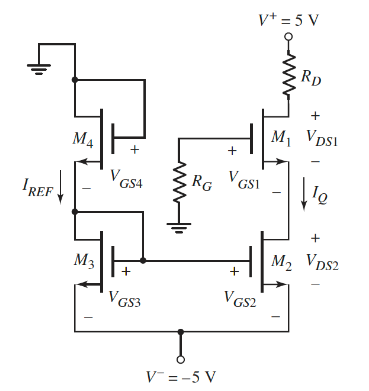
\includegraphics[width = .3\textwidth]{p8.png}
    \end{center}
    \begin{enumerate}
        \item Design the ratio of $K_{n4}/K_{n3}$ such that $V_{GS3} = 2V$
        \begin{align}
            I_{REF} &= I_{REF}\\
            \Rightarrow K_{n4}(V_{GS4}-V_{TN})^2 &= K_{n3}(V_{GS3}-V_{TN})^2\\
            \Rightarrow \frac{K_{n4}}{K_{n3}} &= \frac{(V_{GS3}-V_{TN})^2}{(-V^--V_{GS3}-V_{TN})^2}\\
            \Rightarrow \frac{K_{n4}}{K_{n3}} &= \frac{(2-1)^2}{(-(5)-2-1)^2}\\
            \Rightarrow \frac{K_{n4}}{K_{n3}} &= \boxed{\frac{1}{4}}\\
        \end{align}
        \item Determine $K_{n2}$ such that $I_Q = 100 \mu A$.
        \begin{equation}
            K_{n2} = \frac{I_Q}{(V_{GS2}-V_{TN})^2} = \frac{100\mu A}{1V^2} = \boxed{0.1 \frac{mA}{V^2}}
        \end{equation}
        \item Find $K_{n3}$ and $K_{n4}$ such that $I_{REF} = 200\mu A$ 
        \begin{equation}
            K_{n3} = \frac{200\mu A}{1V^2} = 0.2 \frac{mA}{V^2}
        \end{equation}
        \begin{equation}
            K_{n4} = \frac{0.2}{4} = \boxed{0.05 \frac{mA}{V^2}}
        \end{equation}
    \end{enumerate}
    \newpage
    \item For the transistor in the circuit in the figure below the parameters are $V_{TN} = 0.4V, k_{n}^{'} = 120 \mu A/V^2,$ and $W/L = 25$. Determine $V_{GS}, I_D,$ and $V_{DS}$. Sketch the load line and plot the Q-point.
    \begin{center}
        \begin{circuitikz}[american voltages]
            \draw (0,0) to [short](2.01,0);
            \ctikzset{tripoles/mos style/arrows}s
            \draw (3,0) node[nmos]{};
            \draw (0,0) to [R,l=$14k\Omega$](0,3)
            to [short](3,3)
            to [R, l=$1.2k\Omega$](3,.777);
            \draw (0,0) to [R, l=$6k\Omega$](0,-3)
            to [short](3,-3)
            to [R,l=$0.5k\Omega$](3,-.777);
            \draw (1.5, 3) to[short, -o,l=$+5V$](1.5, 3.5);
            \draw (1.5, -3) to[short, -o,l=$-5V$](1.5, -3.5); node[ground]{};
        \end{circuitikz}
    \end{center}
    \begin{align}
        K_n &= k_{n}^{'} \frac{W}{2L} = 120 \frac{\mu A}{V^2}*12.5 = 1.5 \frac{m A}{V^2}\\
        v_G &= 10V \frac{6k\Omega}{20k\Omega} -5 = -2V\\
        v_{GS} &= v_G - i_DR_D
    \end{align}
    \begin{center}
        Using the information above we can solve for unknowns:
    \end{center}
    \begin{align}
        v_{GS} &= v_G - K_n(v_{GS}- V_{TN})^2(R_S)\\
        \Rightarrow v_{GS} &= -2V - 1.5 \frac{m A}{V^2}(v_{GS}- 0.4V)^2(0.5k\Omega)\\
        \Rightarrow v_{GS} &= -2V - 750\frac{\mu A\cdot\Omega}{V^2}(v_{GS}^2 - 0.8v_{GS} + 0.16V^2)\\
        \Rightarrow v_{GS} &= -2V - .00075v_{GS}^2 + .0006v_{GS} - .00012V\\
        \Rightarrow 0 &= .00075v_{GS}^2 - .0006v_{GS} + 2.00012V\\
        \Rightarrow v_{GS} &= \boxed{1.71V}
    \end{align}
    \begin{center}
        After choosing the correct value of $v_{GS}$ from the quadratic we can move on to solving for the rest of the unknowns:
    \end{center}
    \begin{align}
        i_D &= 1.5 \frac{m A}{V^2}(1.71V - 0.4V)^2\\
        &= \boxed{2.58mA}\\
        v_{DS} &= v_{DD} - (1.2k\Omega+0.5k\Omega)(i_D)\\
        &= \boxed{5.614V}
    \end{align}
    \newpage
    \item The parameters of the transistor in the figures below are $K_n = 0.5 mA/V^2, V_{TN} = 1.2V$, and $\lambda = 0$. Determine $v_{GS}$ and $v_{DS}$ for each transistor when:
    \begin{enumerate}
        \item $\\$
        \begin{center}
            \begin{circuitikz}[american]
                \ctikzset{tripoles/mos style/arrows}
                \draw (0,0) node[ground]{} to [short](.5,0)
                (1.49,0) node[nmos]{}
                (1.49, .78) to [short, -o](1.49, 1.25)node[anchor=south]{$+5V$}
                (1.49, -.78) to [isource,l=$I_Q$,-o](1.49,-2.5) node[anchor=north]{$-5V$};
            \end{circuitikz}
        \end{center}
        \begin{equation}
            v_{GS} = \sqrt{\frac{i_D}{K_n}} + V_{TN}
        \end{equation}
        \begin{enumerate}
            \item $I_Q = 50 \mu A$ 
            \begin{equation}
                v_{GS} = \sqrt{\frac{50 \mu}{.5m}} + 1.2 = \boxed{1.516}
            \end{equation}
            \begin{equation}
                v_{DS} = 5V - (-1.516) = \boxed{6.516}
            \end{equation}
            \item $I_Q = 1 mA$ 
            \begin{equation}
                v_{GS} = \sqrt{\frac{1 m}{.5m}} + 1.2 = \boxed{2.614}
            \end{equation}
            \begin{equation}
                v_{DS} = 5V - (-2.614) = \boxed{7.614}
            \end{equation}
        \end{enumerate}
        \item $\\$
        \begin{center}
            \begin{circuitikz}[american]
                \ctikzset{tripoles/mos style/arrows}
                \draw (0,0) to [short](.5,0)
                (0,0) to [short] (0,.75) to (1.49,.75)
                (1.49,0) node[nmos]{}
                (1.49, .78) to [isource,l=$I_Q$,-o,invert](1.49, 2.5)node[anchor=south]{$+5V$}
                (1.49, -.78) to [short](1.49,-1) node[ground]{};
            \end{circuitikz}
        \end{center}
        \begin{enumerate}
            \item $I_Q = 50 \mu A$ 
            \begin{equation}
                v_{GS} = v_{DS} = \sqrt{\frac{50 \mu}{.5m}} + 1.2 = \boxed{1.516}
            \end{equation}
            \item $I_Q = 1 mA$
            \begin{equation}
                v_{GS} = v_{DS} = \sqrt{\frac{1 m}{.5m}} + 1.2 = \boxed{2.614}
            \end{equation}
        \end{enumerate}
    \end{enumerate}
\end{enumerate}
\end{document}
